\section{Features}

Over all the challege was to understand what makes a vine popular. And for that the there was a need to explore correlations of all the possible abstract midlevel features made available to us because of the rapid development in the fields of Deep machine learning. The main important contribution of machine learning is the ability of computationally extracting abstract higher level representations, which vaguely represent human perception. 

\subsection{Low level Aesthetic Features}:
There are some well known computationally evaluatable aesthetic features like Rule of thirds, Sharp Pixel proportion, Contrast, Simplicity etc \cite{yeh2010personalized}. The parameters basically compute perceptual features of an image based on well know heurestic rules set by photographers. For baseline and comparison, we compare the features with images taken from the dataset from photo.net \cite{datta2008algorithmic}. We only choose images with median ratings of 6 or above on aesthetic scale of 0 to 7. 
Because of the very nature of Vine videos, it was possible to sample 6 images , one for each second of the video, to get a good approximation of the aesthetic quality of the whole video. So in our processing pipeline, we sample one image per second from the 6 second long vine, and then take a median score of the aesthetic parameter across the sampled image. This score is assigned to the whole video to signify the value of that particular aesthetic parameter. 

\begin{table}
\caption{List of Aesthetic parameters computed for highly rated aesthetic images, Popular videos and unpopular videos. Most parameters have no bias towards either popular or unpopular videos}

\resizebox{\linewidth}{!}{%
\begin{tabular}{|l|*{11}{c|}}
  \hline
   Parameter & \multicolumn{2}{|c|}{Aesthetic Images}  &  \multicolumn{2}{|c|}{Popular Vines} & \multicolumn{2}{|c|}{Unpopular Vines} \\ \hline
   \_ & Mean&Median&Mean&Median&Mean&Median\\ \hline
   \ Color Contrast & 51.05 & 30.22 & 29.88 &16.43 & 20.23  & 8.83  \\ \hline
   \ Intensity Balance & 0.11 & 0.08 & 0.16 & 0.13 & 0.17 & 0.14 \\ \hline
   \ Luo Simplicity & 0.009 & 0.005 & 0.013 & 0.012 & 0.015  & 0.014  \\ \hline
   \ Sharp pixel proportion & 0.103 & 0.098 & 0.090 & 0.085 & 0.089  & 0.081  \\ \hline
   \ Image Saturation & 0.943 & 0.974 & 0.672 & 0.678 & 0.615  & 0.646  \\ \hline
   \ Avg. Brightness & 0.148 & 0.141 & 0.137 & 0.130 & 0.139  & 0.124  \\ \hline
   \ Rule of Thirds & 0.879 & 0.899 & 0.883 & 0.883 & 0.878  &0.882  \\ \hline
   \ ROI Proportion & 0.316 & 0.089 & 0.175 & 0.112 & 0.165  & 0.110  \\ \hline
\end{tabular}}

\end{table}

\subsection{ Presence of Faces }:
One important aspect of micro videos is the presence of user as an actor in the video. When you look at viral vine videos, most videos seem to have a lead actor performing a skit. The hypothesis here was that vine has become a social media network, where actors have gained prominence and become a reason for popularity. So we did a small experiment, where we sample one image every second from all the videos collected. Then we calculate the percentage of frames across each video which contained at least one face in it. We use the well tested Viola Jones dectector for frontal and profile face detection \cite{viola2004robust}.

\begin{figure}[!htb]
\centering
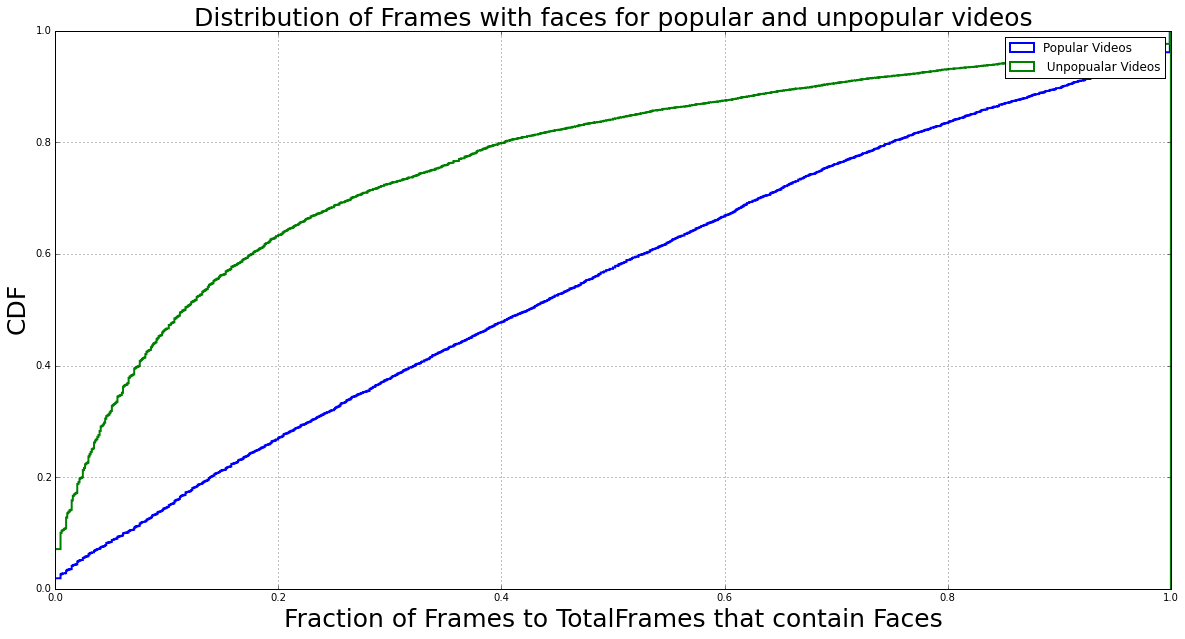
\includegraphics[width=\columnwidth]{plots/FaceCDF}
\caption{\textsl{ CDF for popular and unpopular videos. The CDF signifies the cumulative distribution of percentages of face containing frames in a vine video. The observation here is popular videos tend to have higher percentages than unpopular videos}}
\label{fig:CDF_posts}
\end{figure}

